\chapter{Исследовательская часть}

\section{Технические характеристики}

Технические характеристики устройства, на котором выполнялись замеры времени, представлены далее:

\begin{itemize}
	\item Процессор -- 2 Гц 4‑ядерный процессор Intel Core i5;
	\item Оперативная память -- 16 ГБайт;
	\item Операционная система -- macOS Venura 13.5.2. 
\end{itemize}

\section{Пример работы программы}

% \begin{figure}[h]
% 	\centering
% 	\includegraphics[height=0.4\textheight]{img/exampleProg.png}
% 	\caption{Демонстрация работы программы}
% 	\label{img:demonstration}
% \end{figure}

В данном подразделе представлен пример \ref{lst:LM} работы программы:

\begin{lstlisting}[label=lst:LM,caption=Пример работы программы]
	ivanmamvriyskiy@MacBook-Pro-Ivan-2 main % go run main.go 
	Выберите пункт меню:
	1)Одиночный случай;
	2)Запуск тестов;
	3)Выход из программы.
	1

	Введите размер слайса: 3

	Введите 1 элемент слайса: 1
	Введите 2 элемент слайса: 2
	Введите 3 элемент слайса: 3

	Пирамидальная сортировка: 1 2 3 
	Блинная сортировка: 1 2 3 
	Сортировка перемешиванием: 1 2 3 
\end{lstlisting}

\clearpage
\section{Время выполнения алгоритмов}

В таблицах \ref{tab:tableAsc}, \ref{tab:tableDesc}, \ref{tab:tableRand} предствалены результаты замера времени работы алгоритмов
в зависимости от отсортированности и длины среза. На рисунках 
\ref{img:ascend}, \ref{img:desc}, \ref{img:random} предствалены графики зависимостей времени работы алгоритмов при разной
отсортированности взависимости от длины среза. 

% \begin{figure}[h]
% 	\centering
% 	\includegraphics[height=0.31\textheight]{img/tableAsc.png}
% 	\caption{Время выполнения работы алгоритма при отсортированном по возрастанию срезе.}
% 	\label{img:Tableasc}
% \end{figure}

\begin{table}[!ht]
    \centering
    \caption{\label{tab:tableAsc} Время выполнения работы алгоритмов при отсортированном по возрастанию срезе
    в зависимости от длины среза(нс).}
    \begin{tabular}{|r|r|r|r|r|}
    \hline
        Длина среза & Блинная & Пирамидальная & Перемешиванием   \\ \hline
        10 & 400 & 700 & 400   \\ \hline
        100 & 14 000 & 6 300 & 9 100   \\ \hline
        200 & 52 000 & 13 700 & 32 100   \\ \hline
        300 & 114 500 & 21 800 & 66 800   \\ \hline
        400 & 192 500 & 26 900 & 97 100   \\ \hline
        500 & 261 700 & 34 800 & 147 700   \\ \hline
        600 & 331 000 & 44 300 & 201 100   \\ \hline
        700 & 394 700 & 44 800 & 221 400   \\ \hline
        800 & 445 000 & 47 900 & 251 800   \\ \hline
        900 & 472 800 & 46 300 & 269 100   \\ \hline
        1000 & 575 300 & 52 700 & 322 700   \\ \hline
        2000 & 2 347 800 & 120 600 & 1 292 500   \\ \hline
        3000 & 5 260 300 & 192 300 & 2 858 500   \\ \hline
        4000 & 9 207 500 & 277 400 & 5 126 600   \\ \hline
        5000 & 14 667 500 & 340 100 & 8 006 700  \\ \hline
    \end{tabular}
\end{table}

% \begin{figure}[h]
% 	\centering
% 	\includegraphics[height=0.30\textheight]{img/tableDesc.png}
% 	\caption{Время выполнения работы алгоритма при отсортированном по убыванию срезе.}
% 	\label{img:TableDesc}
% \end{figure}

\begin{table}[!ht]
    \centering
    \caption{\label{tab:tableDesc} Время выполнения работы алгоритмов при отсортированном по убыванию срезе
    в зависимости от длины среза(нс).}
    \begin{tabular}{|r|r|r|r|r|}
    \hline
        Длина среза & Блинная & Пирамидальная & Перемешиванием   \\ \hline
        10 & 100 & 300 & 100   \\ \hline
        100 & 6 500 & 43 00 & 4 000   \\ \hline
        200 & 25 200 & 6 400 & 21 400   \\ \hline
        300 & 65 200 & 15 800 & 45 800   \\ \hline
        400 & 104 600 & 22 800 & 75 500   \\ \hline
        500 & 171 600 & 40 800 & 106 700   \\ \hline
        600 & 237 100 & 26 300 & 184 600   \\ \hline
        700 & 299 200 & 51 500 & 159 400   \\ \hline
        800 & 381 100 & 54 100 & 276 600   \\ \hline
        900 & 486 100 & 72 500 & 313 500   \\ \hline
        1000 & 566 900 & 69 900 & 336 100   \\ \hline
        2000 & 2 453 600 & 127 300 & 1 342 100   \\ \hline
        3000 & 5 321 100 & 248 500 & 2 926 000   \\ \hline
        4000 & 9 185 700 & 264 500 & 5 037 100   \\ \hline
        5000 & 15 129 900 & 350 900 & 8 189 500  \\ \hline
    \end{tabular}
\end{table}

% \begin{figure}[h]
% 	\centering
% 	\includegraphics[height=0.30\textheight]{img/tableRand.png}
% 	\caption{Время выполнения работы алгоритма при рандомном расположении чисел в срезе.}
% 	\label{img:TableRandom}
% \end{figure}

\begin{table}[!ht]
    \centering
    \caption{\label{tab:tableRand} Время выполнения работы алгоритмов при рандомном расположении чисел в срезе
    в зависимости от длины среза(нс).}
    \begin{tabular}{|r|r|r|r|r|}
    \hline
        Длина среза & Блинная & Пирамидальная & Перемешиванием  \\ \hline
        10 & 500 & 100 & 400  \\ \hline
        100 & 11 500 & 700 & 4 900  \\ \hline
        200 & 42 300 & 1 900 & 22 700  \\ \hline
        300 & 99 000 & 2 500 & 44 400  \\ \hline
        400 & 131 500 & 2 200 & 65 200  \\ \hline
        500 & 243 800 & 3 100 & 114 400  \\ \hline
        600 & 354 300 & 5 100 & 140 700  \\ \hline
        700 & 387 500 & 3 500 & 159 000  \\ \hline
        800 & 515 500 & 5 600 & 232 200  \\ \hline
        900 & 678 600 & 4 600 & 283 100  \\ \hline
        1000 & 808 800 & 5 800 & 331 800  \\ \hline
        2000 & 3 413 700 & 10 200 & 1 331 300  \\ \hline
        3000 & 6 737 100 & 14 800 & 2 869 200  \\ \hline
        4000 & 11 649 900 & 19 600 & 5 008 700  \\ \hline
        5000 & 19 142 300 & 36 300 & 8 176 300 \\ \hline
    \end{tabular}
\end{table}

\begin{figure}[h]
	\centering
	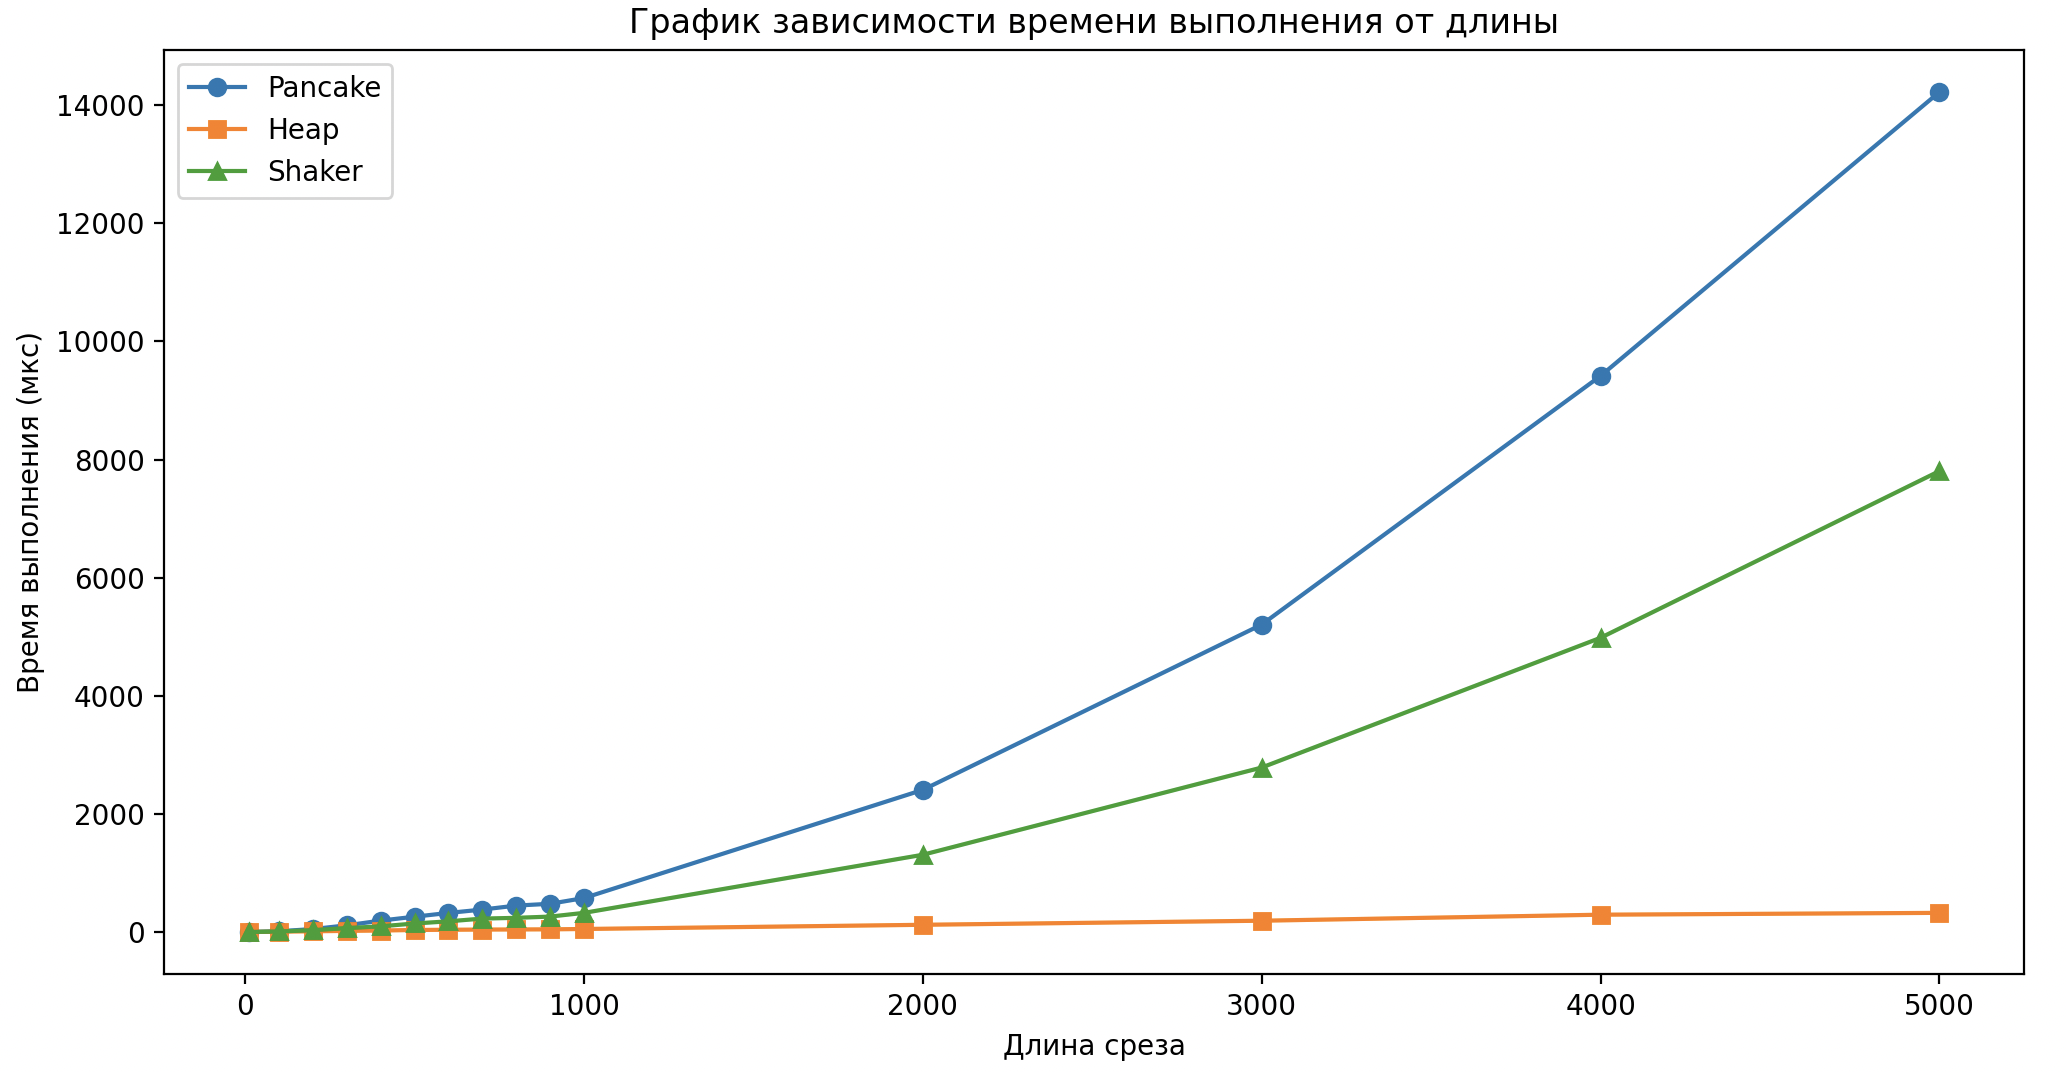
\includegraphics[height=0.35\textheight]{img/ascend.png}
	\caption{Время выполнения работы алгоритма при отсортированном по возрастанию срезе
    в зависимости от длины среза.}
	\label{img:ascend}
\end{figure}

\begin{figure}[h]
	\centering
	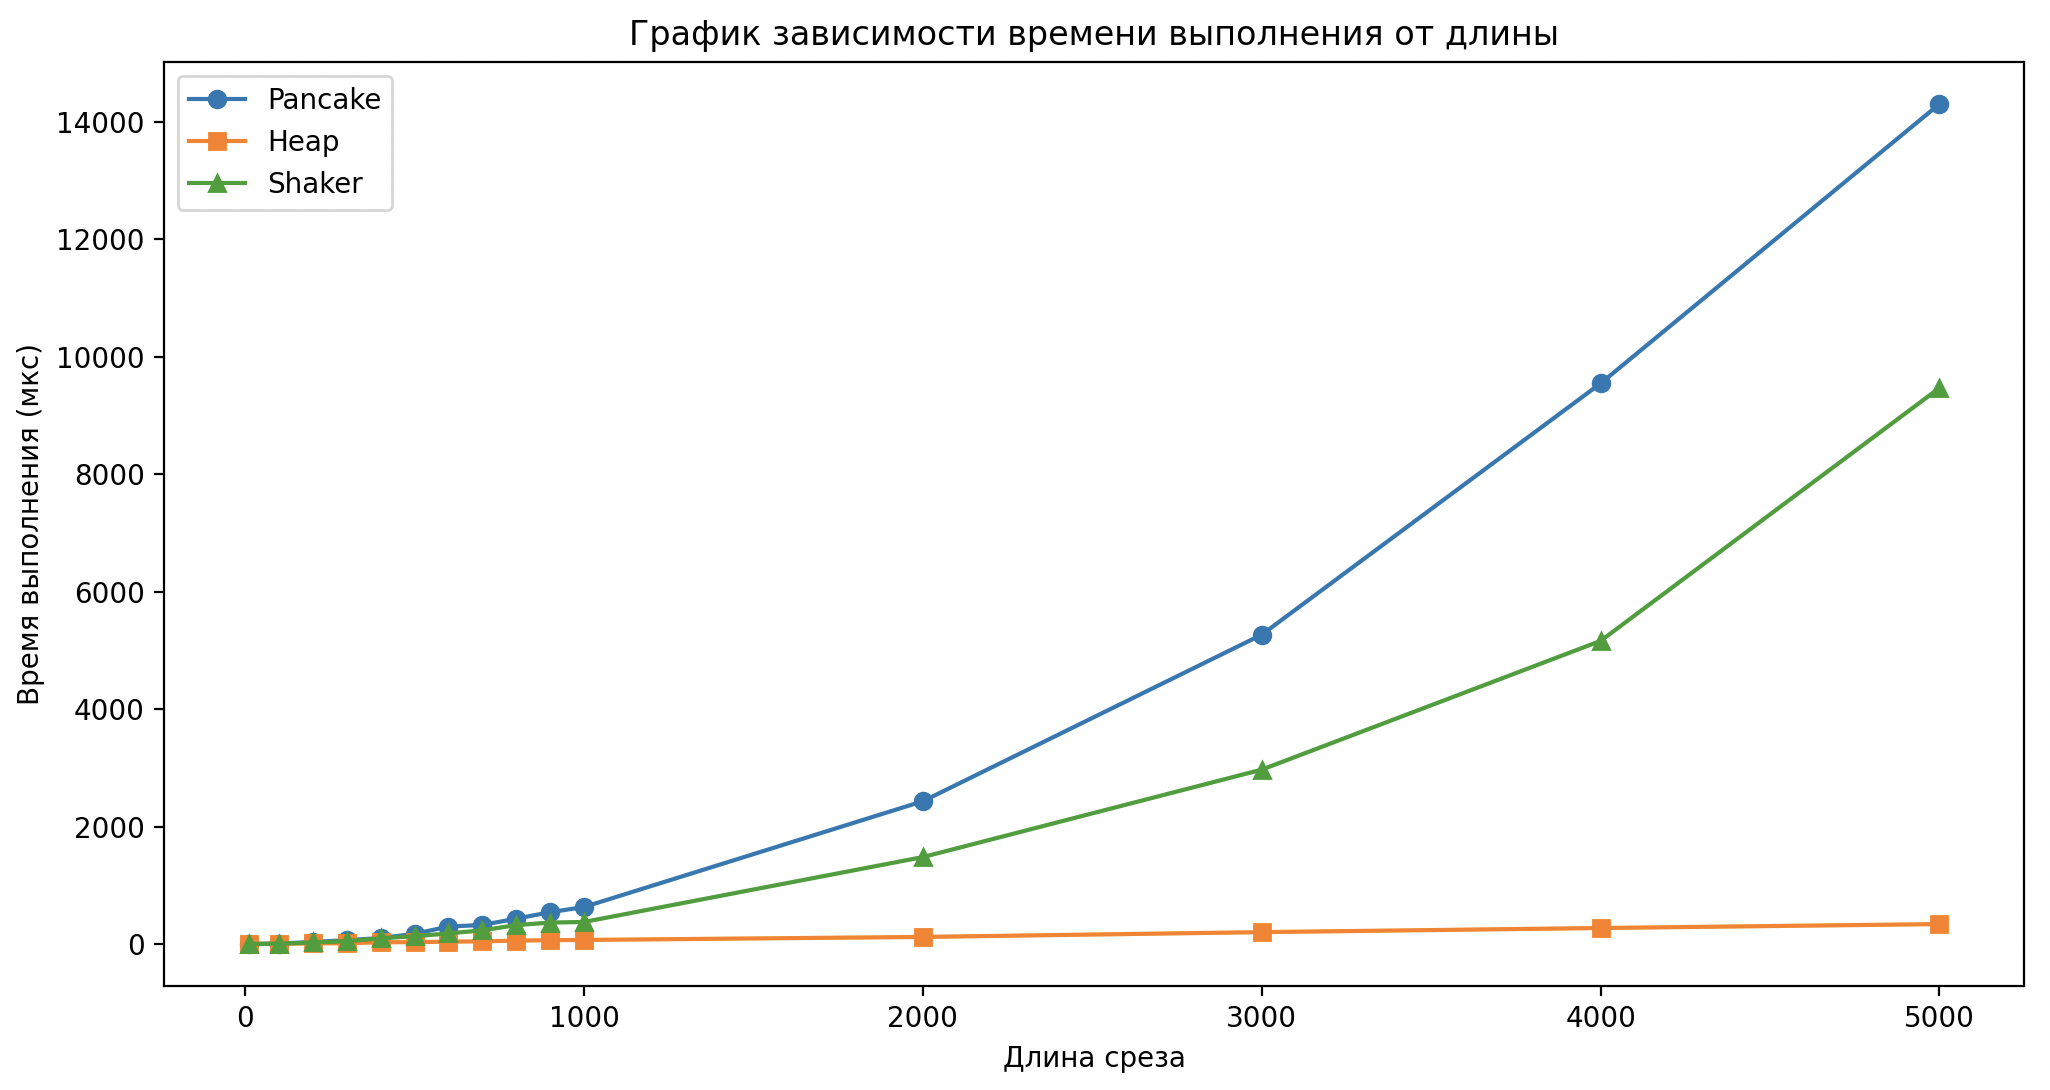
\includegraphics[height=0.35\textheight]{img/descend.png}
	\caption{Время выполнения работы алгоритма при отсортированном по убыванию срезе
    в зависимости от длины среза.}
	\label{img:desc}
\end{figure}

\begin{figure}[h]
	\centering
	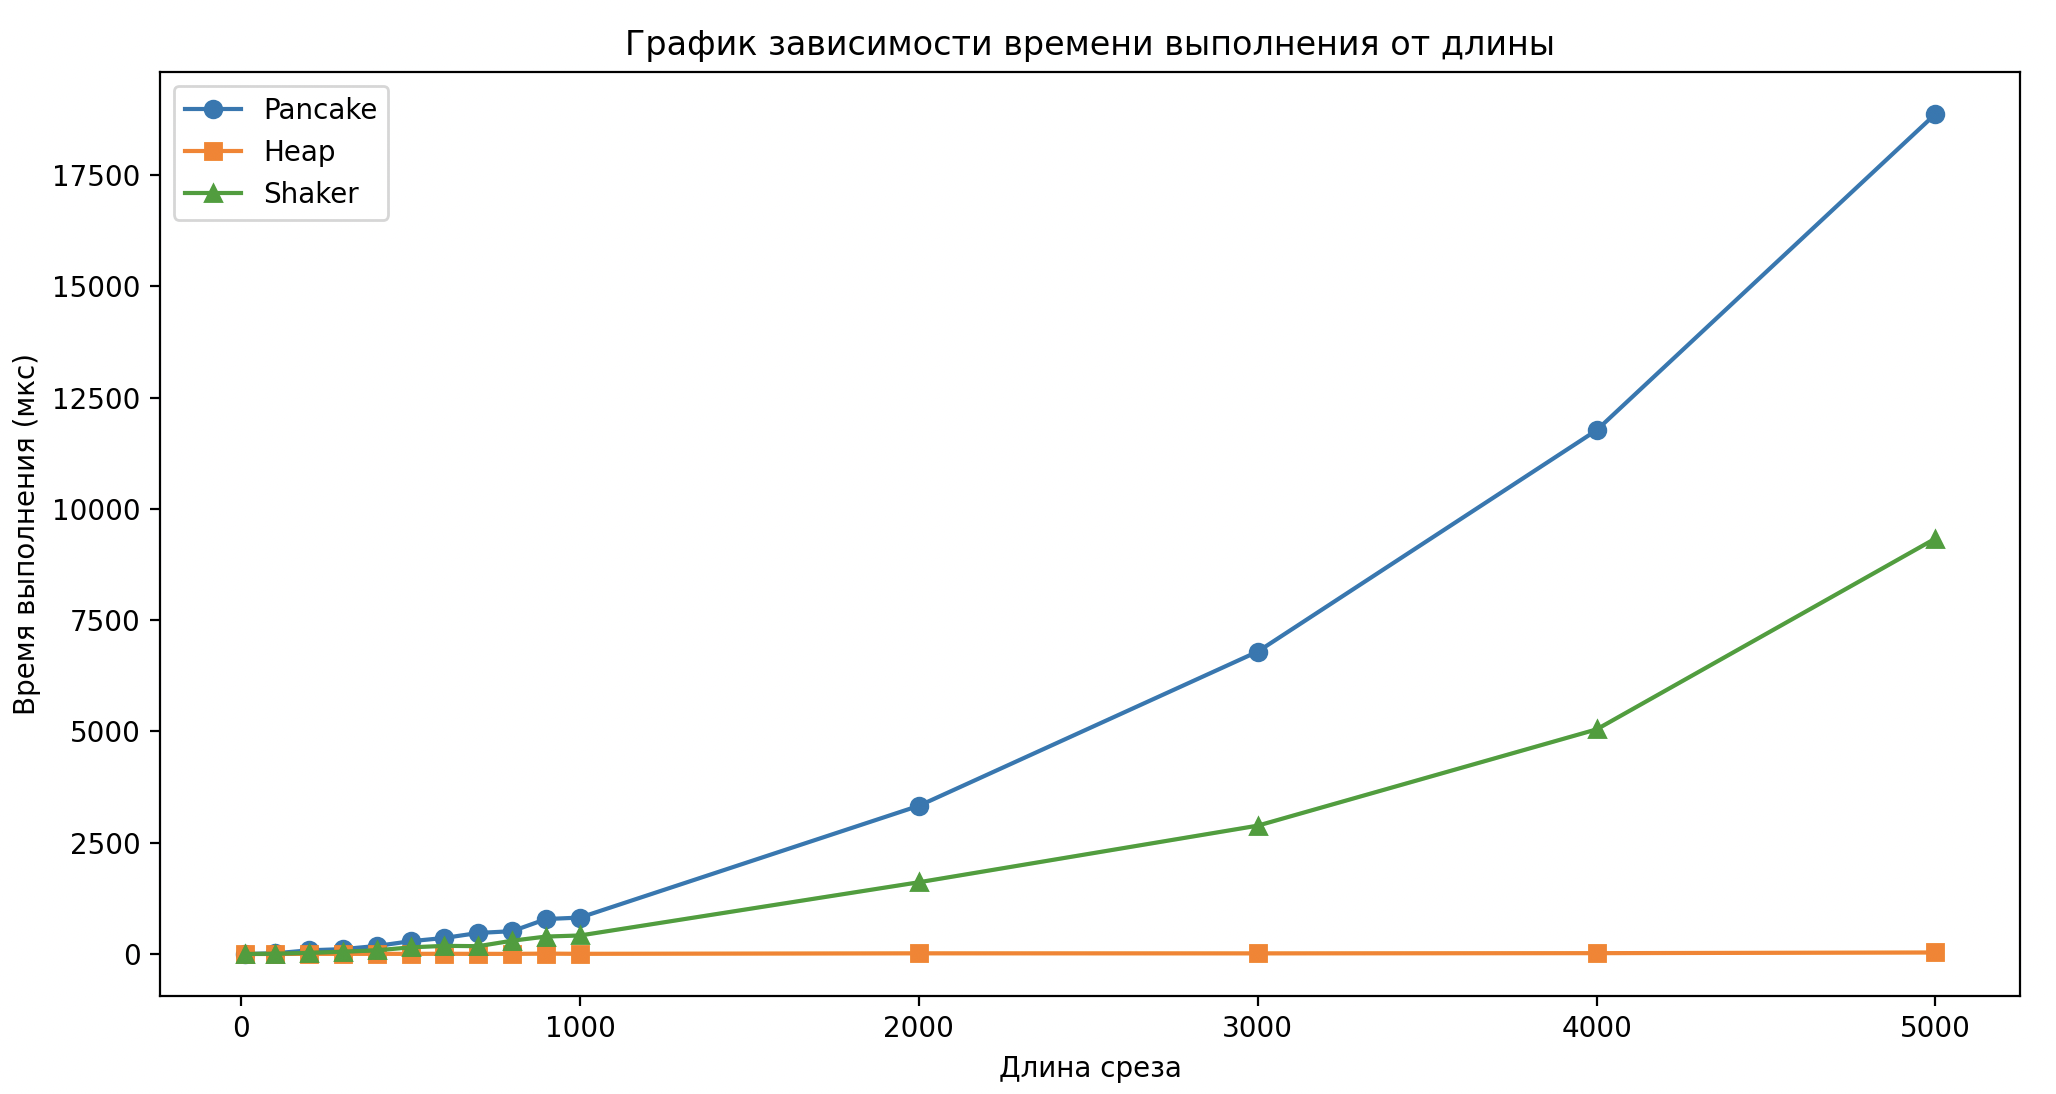
\includegraphics[height=0.35\textheight]{img/random.png}
	\caption{Время выполнения работы алгоритма при рандомном расположении чисел в срезе
    в зависимости от длины среза.}
	\label{img:random}
\end{figure}

\clearpage

По результатам эксперимента можно сделать следующие выводы:
\begin{itemize}[left=\parindent]
    \item Алгоритм блинной сортировки работает 
	медленнее всех при любых способах расположения элементов в последовательности, а пирамидальный алгоритм
	сортировки -- быстрее всех. 
	\item Любой из алгоритмов быстрее всего работает при отсортированной по 
	возрастанию последовательности.
	\item Блинная сортировка быстрее всего работает при отсортированной последовательности
	по возрастанию, так как не происходит двойного поворота при нахождении индекса максимального 
	числа не равного текущей длине. 
	\item Пирамидальная сортировка при любом расположении элементов происходит примерно одинаково.
	Выигрыш по времени происходит в случаях, когда максимальное значение находится в родительской ячейке, 
	так как не происходит обмена.
	\item Сортировка перемешиванием быстрее выполнятеся, когда последовательность 
	отсортирована по возрастанию, так как не происходит перетаскивания максимальных
	и минимальных значений. Дольше всего выполнеятся, когда последовательность 
	отсортирована по убыванию, так как на каждом шаге происходит протаскивание максимальных и
	минимальных значений.
\end{itemize}


\section{Вывод}

Таким образом, для более быстрой сортировки последовательности независимо от расположения
в ней элементов необходимо использовать пирамидальную сортировку. 
